\section{Технический проект}
\subsection{Общая характеристика организации решения задачи}

Необходимо спроектировать и разработать приложение, которое обеспечит функционирование СКУД на круизном лайнере AIDABlu.

Приложение представляет собой панель управления для работы с данными в базе данных системы. Панель содержит текстовую и графическую информацию (TreeView).

Приложение является десктопным, т.е. располагается и запускается внутри лишь одной операционной системы. Каждое окно приложения (за исключением главного) – это панель управления для конкретной таблицы базы данных. Приложение разработано на языке Python v3.10. Управление данными БД реализовано с помощью библиотеки sqlite3 и SQL -- языка структурированных запросов к базе данных.

\subsection{Общие сведения о программно-информационной системе}

Полное наименование системы: Программное обеспечение для системы контроля и управления доступом на круизном судне.

Краткое обозначение системы: \textquotedbl СКУД на круизном лайнере \textquotedbl.

Описание системы: \textquotedbl СКУД на круизном лайнере \textquotedbl предназначена для корпораций, организующих круизные путешествия, предоставляя им платформу для удобного контроля и управления данными всей бизнес-системы круизного лайнера на время поездки. Система создана для обеспечения комфортной и безопасной поездки каждого пассажира и функционирования в форс-мажорных ситуациях.

Условия эксплуатации: \textquotedbl СКУД на круизном лайнере \textquotedbl предназначена для использования как в нормальных, так и в чрезвычайных условиях работы.

Архитектура системы: Программное обеспечение основано на десктопной архитектуре, используя современные технологии разработки, включая TKinter и CustomTkinter для интерфейса пользователя и sqlite3 для реализации запросов к БД. Система использует базу данных SQLite.

Технологии и инструменты: В разработке использовались tkinter, customtkinter, sqlite3, asyncio, time

\subsection{Обоснование выбора технологии проектирования}

\subsubsection{Описание используемых технологий и языков программирования}

В процессе разработки приложения используются программные средства и языки программирования. Каждое программное средство и каждый язык программирования применяется для круга задач, при решении которых они необходимы.

\subsubsection {tkinter}
Выбор tkinter для разработки интерфейса пользователя обосновывается его простотой и кроссплатформенной поддержкой, а также минимальными требованиями к интерфейсу в пользу быстродействия. 

Пакет tkinter («интерфейс Tk») - это интерфейс Python для создания GUI. Tkinter доступен на большинстве платформ Unix, включая macOS, а также на системах Windows.

Tkinter входит в состав большинства инсталляций Python, что делает его легкодоступным для разработчиков, которые хотят создавать приложения с графическим интерфейсом, не требуя дополнительных инсталляций или библиотек.

\subsubsection {customtkinter}
Выбор customtkinter для Front-End обосновывается его расширенным функционалом по сравнению с tkinter. Customtkinter предлагает большой список параметров для настройки виджетов и является полностью совместимым с элементами tkinter.

CustomTkinter - это библиотека пользовательского интерфейса для настольных компьютеров на основе Tkinter, которая обеспечивает современный вид и полностью настраиваемые виджеты.

\subsubsection {SQLite}
Выбор SQLite в качестве системы управления базами данных также обосновывается его удобством как на этапе проектирования, так и на этапе реализации.

SQLite - это библиотека на языке C, которая предоставляет легкую дисковую базу данных, не требующую отдельного серверного процесса и позволяющую обращаться к базе данных с помощью нестандартного варианта языка запросов SQL. Некоторые приложения могут использовать SQLite для внутреннего хранения данных. Также можно создать прототип приложения с использованием SQLite, а затем перенести код на более крупную базу данных, такую как PostgreSQL или Oracle.

\subsubsection {asyncio и time}
Модули asyncio и time были использованы для актуализации работы системы в реальном времени и многопоточном режиме.


\subsubsection{Язык структурированных запросов к базе данных SQL}
SQL - это стандартизированный язык программирования, который используется для управления реляционными базами данных и выполнения различных операций над данными в них. 

SQL используется для следующего:
\begin{itemize}
	\item изменение структуры таблиц данных и индексов базы данных;
	\item добавление, обновление и удаление строк данных;
	\item извлечение подмножеств информации из реляционных систем управления базами данных (РСУБД).
\end{itemize}


\subsubsection{Язык программирования Python}

\paragraph{Достоинства языка Python}
Python - очень продуктивный язык. Благодаря простоте Python разработчики могут сосредоточиться на решении проблемы. Написание кода экономит время и освобождает его для более ёмкой работы с другими составляющими проекта.

Python поставляется под лицензией OSI с открытым исходным кодом. Это делает его свободным для использования и распространения. Можно загружать исходный код, изменять его и даже распространять свою версию Python. Это полезно для организаций, которые хотят изменить некоторые специфические функции и использовать свою версию для разработки.

Стандартная библиотека Python огромна, в ней можно найти практически все функции, необходимые для решения любой задачи. Таким образом, не придется зависеть от внешних библиотек.

Во многих языках, таких как C/C++, для запуска программы на разных платформах необходимо изменять код. С Python дело обстоит иначе. Вы пишете один раз и запускаете программу в любом месте.

\subsection{Проектирование пользовательского интерфейса}
На основании требований к пользовательскому интерфейсу, представленных в пункте 2.3 технического задания, был разработан графический интерфейс десктопного приложения с применением python tkinter и customtkinter Этот процесс подчеркивает важность интуитивно понятного и эффективного взаимодействия с пользователем. Разработанный интерфейс ориентирован на обеспечение легкости в использовании и интуитивного понимания функционала приложения, предоставляя пользователю простое и эффективное взаимодействие с приложением.

\begin{enumerate}
	\item Навигация по таблицам с данными. Реализация функции навигации на основе полей psr\underline{ }btn, psr\underline{ }ua\underline{ }btn, drs\underline{ }btn, rms\underline{ }btn, pns\underline{ }btn, acs\underline{ }btn.

	\item Панель управления для каждой из таблиц с данными. Диверсификация интерфейсов происходит на основе метода show\underline{ }table класса Controller.

	\item Отображение текущей таблицы с данными в реальном времени. Актуальность этого графического элемента (дерева) поддерживается за счёт методов TreeRefresh и TreeCreate класса Controller.

	\item Воздействие на внесённые данные базы. Добавление, изменение или удаление элементов реализованы в методах add\underline{ }element, update\underline{ }element и delete\underline{ }element класса Tables соответственно, внутри которых формирование строк запросов к БД реализовано с помощью класса Utils.

	\item Навигация и лёгкий поиск среди элементов среди данных. Пользователь может переходить по элементам последовательно (метод MoveTo класса Controller), или же использовать отдельное текстовое поле для метода search\underline{ }element класса Tables, перейдя сразу к искомому элементу таблицы.

	\item Отображение локального времени. Учитывая специфику проекта -- систему для круизного лайнера, учтено, что часовой пояс может измениться во время путешествия. На уровне python и SQL была установлена привязка к локальному времени (localtime), а функционал часов запущен в асинхронном потоке во избежание ошибок и помех работы основной системы.

	\item Запрос доступа к двери. На основе правил, прописанных в полях Комнаты, к которой привязана выбранная Дверь, в отдельном окне отображается информация о том, есть ли у Пассажира доступ к этой Двери.
\end{enumerate}

\begin{figure} [H]
	\centering
	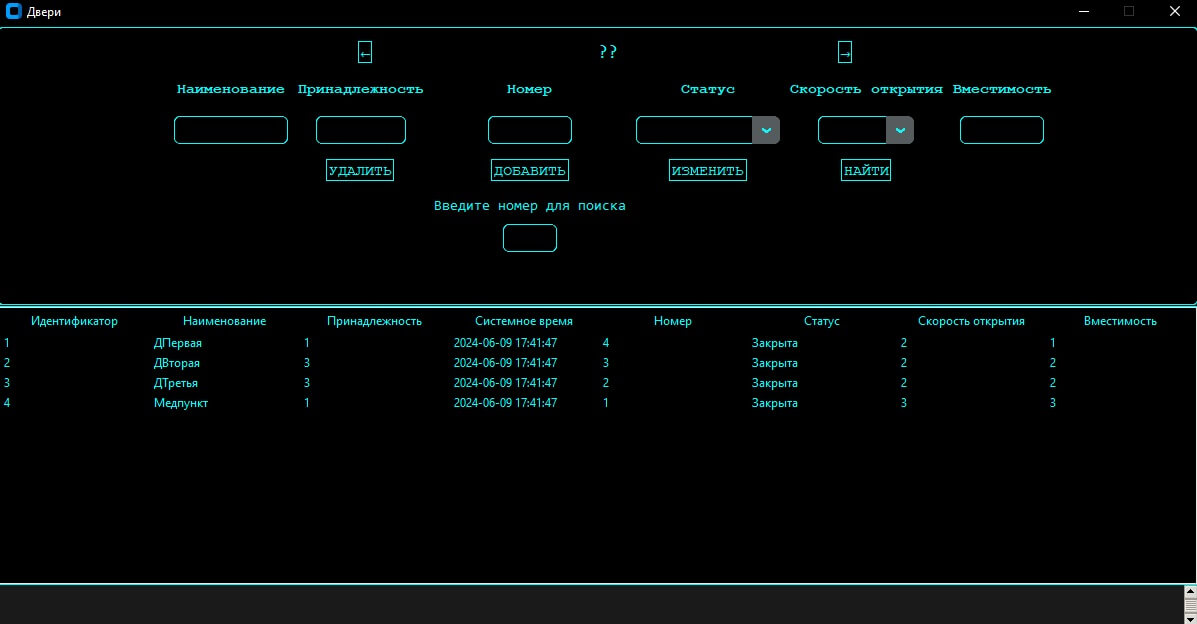
\includegraphics[width=1.05\linewidth]{images/Example2}
	\caption{Модели интерфейса <<Панель управления для каждой из таблиц с данными>> и <<Отображение текущей таблицы с данными в реальном времени>>}
	\label{fig:example2}
\end{figure}

На рисунке ~\ref{fig:example2} изображена модель интерфейса панели управления данными.

Процесс изменения данных максимально упрощён и включает следующие шаги:

\begin{enumerate}
	\item В главном меню пользователь выбирает поле с названием необходимого ему вида данных.

	\item В появившемся окне пользователь находит нужный ему элемент посредством <<Пролистывания>> или посредством поиска по идентификатору, при нажатии на соответствующие подписанные поля.

	\item Пользователь изменяет некоторые данные в полях элемента и выбирает опцию <<Изменить>>, если ему нужно было редактировать элемент, или <<Удалить>>, если была необходимость удалить элемент.

	\item Если пользователю необходимо добавить элемент, он должен заполнить поля ввода: наименование, принадлежность, номер, статус, скорость открытия, вместимость (В случае работы с данными о дверях) и выбрать опцию <<Добавить>>.

	\item На последнем этапе, если все обязательные поля были заполнены данными корректного формата, пользователь получает сообщение об успешном проведении операции и она выполняется.
\end{enumerate}

На рисунке ~\ref{fig:example1} изображена модель интерфейса панели при изменении данных элемента.

\begin{figure} [H]
	\centering
	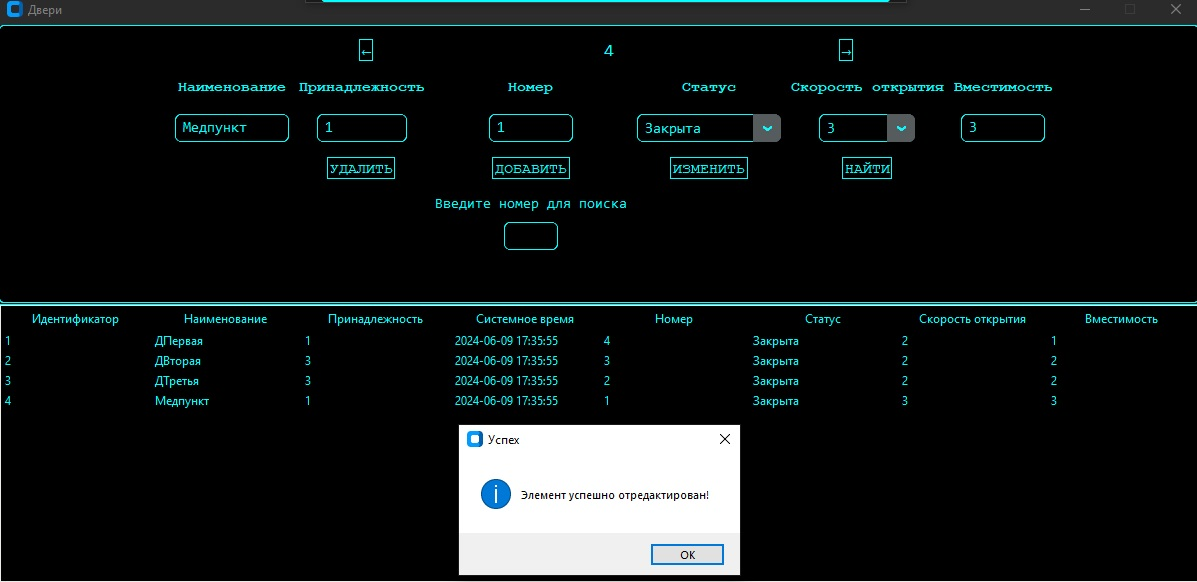
\includegraphics[width=1.05\linewidth]{images/Example1}
	\caption{Модель интерфейса <<Изменение данных элемента>>}
	\label{fig:example1}
\end{figure}

Процесс получения информации о доступе является еще более простым и состоит из следующих этапов:

\begin{enumerate}
	\item В главном меню пользователь выбирает опцию <<Проверка доступа>>.

	\item В появившемся окне пользователь с помощью переключателя выбирает нужную ему группу поиска среди пассажиров - таблицу <<Пассажиры>> или <<Дети>>.

	\item Пользователь вводит идентификаторы пассажира и двери в поля \textquotedbl Пассажир \textquotedbl и \textquotedbl Дверь \textquotedbl соответственно и выбирает опцию <<Проверить доступ>>.

	\item На последнем этапе, если все обязательные поля были заполнены данными корректного формата и в БД содержатся данные о предоставленном/отказанном доступе, пользователь получает сообщение о том, есть ли у указанного пассажира доступ к указанной двери.
\end{enumerate}

На рисунке ~\ref{fig:example3} изображена модель интерфейса <<Запрос доступа к двери>>.

\begin{figure} [H]
	\centering
	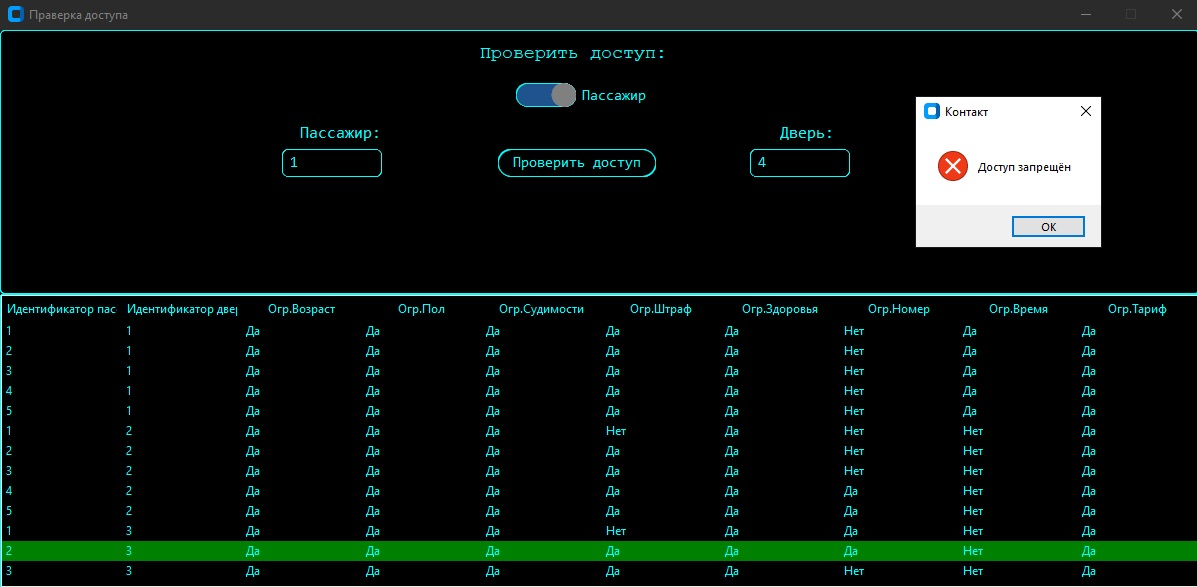
\includegraphics[width=1.05\linewidth]{images/Example3}
	\caption{Модель интерфейса <<запрос доступа к двери>>}
	\label{fig:example3}
\end{figure}


\subsection{Диаграмма компонентов}
Диаграмма компонентов описывает особенности физического представления разрабатываемой системы. Она позволяет определить архитектуру системы, установив зависимости между программными компонентами, в роли которых может выступать как исходный, так и исполняемый код. Основными графическими элементами диаграммы компонентов являются компоненты, интерфейсы, а также взаимосвязи между ними. На рисунке \ref{fig:commonscheme5} изображена диаграмма компонентов для проектируемой системы. Детальное и глубокое понимание этих взаимосвязей критически важно для успешного создания и функционирования программной системы.

Каждый компонент системы играет важную роль в обеспечении её общей эффективности и надежности.
Подход, основанный на стратегическом планировании, способствует оптимизации этих взаимодействий и повышает вероятность успешной реализации и эксплуатации системы в целом.
\begin{landscape}
\begin{figure} [H]
	\centering
	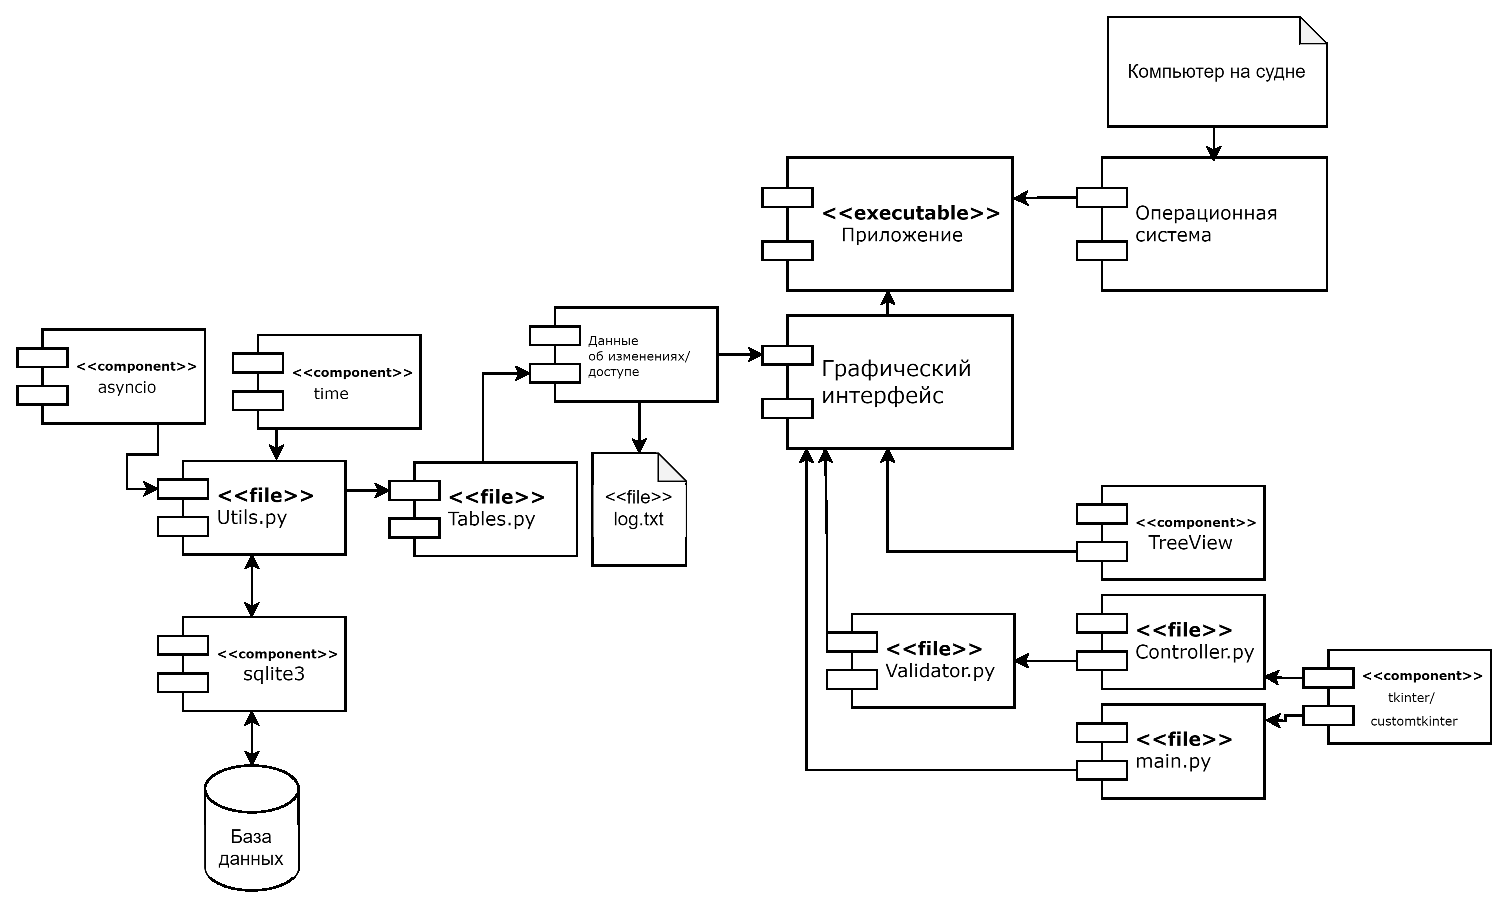
\includegraphics[width=1\linewidth]{images/CompDiag}
	\caption{Диаграмма компонентов}
	\label{fig:commonscheme5}
\end{figure}
\end{landscape}
Она является хорошим средством для показа маршрутов перемещения объектов и компонентов в распределенной системе.

\subsection{Описание архитектуры приложения}

Архитектура приложения, реализованная в рамках текущей работы, базируется на модели MVC (Model-View-Controller). Этот паттерн был избран из-за его способности к эффективному распределению функциональных обязанностей между структурными компонентами системы, а также способствованию упрощению процессов разработки и тестирования.

MVC реализован следующим образом:

1. Модель (Model) и контроллер (сontroller): эти компоненты обеспечивают управление бизнес-логикой и обработку данных, а также связь между пользовательским интерфейсом и базой данных.

2. Представление (View): реализовано через интерфейс пользователя, использующий пакеты tkinter, customtkinter и treeview, и отвечающий за визуализацию информации и интерактивное взаимодействие с пользователем.

Ключевым аспектом в управлении данными является использование системы управления базами данных SQLite. Этот выбор был обусловлен высокой надежностью SQLite, её устойчивостью к атакам и гибкостью в обработке сложных запросов, что имеет критическое значение для эффективного функционирования.

Применение архитектуры MVC принесло следующие ключевые преимущества:

\begin{itemize}
	\item четкое разделение обязанностей: эффективное разграничение между пользовательским интерфейсом (класс main.py и controller.py) логикой запросов (tables.py) значительно упрощает процесс разработки и последующей поддержки системы;
	\item гибкость и масштабируемость: благодаря MVC, архитектура приложения легко адаптируется и масштабируется, что позволяет разработчикам
	модифицировать или расширять отдельные части системы без влияния на другие;
	\item упрощение тестирования: независимость компонентов архитектуры MVC облегчает процедуру тестирования, позволяя проводить её для каждого элемента в отдельности.
\end{itemize}

Такой подход устанавливает предпочтительную форму записи организации функционала и способ его использования в тестировании. Он обеспечивает создание надежной, гибкой и масштабируемой системы, а также применим как в крупных, так и в малых проектах.

\subsubsection{Модули}
В системе представлены следующие модули:
\begin{enumerate}
	
	\item Модуль asyncio для организации работы системного времени в отдельном потоке.
	\item Модуль re включается для работы с регулярными выражениями для задания правил написания, валидации полей.
	\item Модуль sqlite3 используется для организации подключения и запросов к базе данных.
	\item Для создания интерфейса пользователя используются модули tkinter, customtkinter и treeView. TreeView необходим для отображения виджета древа таблицы в реальном времени,  customtkinter - для основного интерфейса приложения, а tkinter - для служебного упорядочивания элементов интерфейса customtkinter и treeview.
\end{enumerate}

\subsubsection{Классы}
В системе представлены следующие классы:
\begin{enumerate}

	\item main.py - в этом классе прописан интерфейс главного меню с последующей передачей вводимых данных в другие компоненты.
	
	\item Utils.py - служебный класс, внутри которого реализованы функции запросов к базе данных, асинхронное обновление системного времени(Например, подключение к БД - create\underline{ }connection(), чтение - read\underline{ }single\underline{ }row(), запрос - execute\underline{ }query() и т.д.).
	
	\item Validator.py - служебный класс для задания правил написания (валидации). Необходим для проверки корректности вводимых данных(Например, метод FKValid() - для валидации внешних ключей, overvalidation() для дополнительной проверки корректности перед валидацией).
	
	\item Controller.py - в этом классе прописан интерфейс панели управления таблицами данных с последующей передачей вводимых данных в другие компоненты, а также выводом полученных данных на экран.
	
	\item Tables.py - служебный класс, созданный для формирования запросов к БД. Вся логика взаимодействия с данными внутри базы, таким как добавление - add\underline{ }element(), удаление - delete\underline{ }element() и т.д., содержится в этом классе.

\end{enumerate}